
\chapter{Cross-validation for unsupervised learning}

The problem unsupervised learning (UL) tries to to address is this: given some
data, describe its distribution. Many estimation problems can be cast as
unsupervised learning, including mean estimation, density estimation, and
linear regression. However, more commonly unsupervised learning refers to
either clustering or manifold learning. A canonical example is principal
components analysis (PCA). In PCA, we are given some high-dimensional data,
and we look for a lower-dimensional subspace that explains most of the
variation in the data. The lower-dimensional subspace describes the
distribution of the data. In clustering, the estimated cluster centers give us
information about the distribution of the data. The output of every UL method
is a summary statistic designed to convey information about the process which
generated the data.

Many UL problems involve model selection. For example, in principal components
analysis we need to choose how many components to keep. For clustering, we
need to choose the number of clusters in the data. Many manifold learning
techniques require choosing bandwidth or a kernel. Often in these contexts,
model-selection is done in an ad-hoc manner. Rules of thumb and manual
inspection guide most choices for how many components to keep, how many
clusters are present, and what is an appropriate kernel. Such informal
selection rules can be problematic when different researches come to different
conclusions about what the right model is. Moreover, even when there is an
obvious ``natural'' model to human eyes, it may be hard to pick out in
computer-automated analysis. For objectivity and efficiency, it is desirable to have a well-specified automatic model selection procedure.

For concreteness, in this chapter we focus on principal components, though
many of the ideas generalize to other methods. We suppose that the data,
$\mX$, is an $n \times p$ matrix generated according to the signal-plus-noise
model $\mX = \sqrt{n} \mU \mD \mV^\trans + \mE$. We consider the first term to
be the ``signal'' matrix, and the second term to be ``noise''. Often the
signal term is a low-rank product. Our goal is to estimate the this term as
best as possible by truncating the singular value decomposition (SVD) of
$\mX$. Here ``best'' means with respect to the metrics introduced in
Chapter~\ref{C:intrinsic-rank}. We are interested in the model selection
problem where each model is defined by the number of terms we keep from the
SVD of $\mX$.

We would like our model selection procedure to be non-parametric, if possible.
To work in a variety of contexts, the selection procedure cannot assume
Gaussianity or independence across samples. We would like the procedure to be
driven by the empirical distribution of the data. Cross-validation (CV) is a
popular approach to model selection that generally meets these criteria.
Therefore, we seek to adapt CV to our purposes.

CV prescribes dividing a data set into a ``test'' set and a
``train'' set, fitting a model to the training set, and then evaluating the
model's performance on the test set. We repeat the fit/evaluate procedure
multiple times over different test/train partitions, and then average over all
replicates. Traditionally, the partitions are chosen so that each datum occurs
in exactly one test set. As for terminology, for a particular replicate the
test set is commonly referred to as the held-out or left-out set, and likewise
the train set is often called the held-in or left-in set.

Most often, cross-validation is applied in supervised contexts. In supervised
learning (SL) the data consists of a sequence of $(\vx, \vy)$
predictor-response pairs. Broadly construed, the goal of supervised learning
is to describe the conditional distribution of $\vy$ given $\vx$. This is
usually for prediction or classification.  In the supervised context, for a 
particular CV replicate there are four parts of data:
\[
    \left(
    \begin{matrix}
        \mX_\train & \mY_\train \\
        \mX_\test  & \mY_\test
    \end{matrix}
    \right).
\]
Implicit in the description of cross-validation is that the replicates use
$\mX_\test$ to predict $\mY_\test$. So, the held-in data looks like
\[
    \left(
    \begin{matrix}
        \mX_\train & \mY_\train \\
        \mX_\test  & \missing
    \end{matrix}
    \right).
\]
We extrapolate from $\mX_\test$ to predict $\mY_\test$.

It is not immediately obvious how to apply cross-validation to unsupervised
learning.  In unsupervised learning there is no $\mY$; we instead have the 
two-way partition
\[
    \left(
    \begin{matrix}
        \mX_\train \\
        \mX_\test
    \end{matrix}
    \right).
\]
There is nothing to predict!  Renaming $\mX$ to $\mY$ does not make the
problem any better, for then the division becomes:
\[
    \left(
    \begin{matrix}
        \mY_\train \\
        \mY_\test
    \end{matrix}
    \right),
\]
with holdin
\[
    \left(
    \begin{matrix}
        \mY_\train \\
        \missing
    \end{matrix}
    \right).
\]
There is nothing to extrapolate from to predict $\mY_\test$.  For 
cross-validation to work in unsupervised learning, we need to consider
more general holdouts.

We look at two different types of holdouts in this chapter. The first, due to
Wold, is ``speckled'': we leave out random elements of the matrix $\mX$ and
use a missing data algorithm like expectation-maximization (EM) for
prediction. The second type of holdout is ``blocked''. This type, due to
Gabriel, randomly partitions the columns of $\mX$ into ``predictor'' and
``response'' sets and then performs the SL version of cross-validation.

\section{Assumptions, and notation}\label{S:ucv-assumptions-notation}

We will generally assume we have data $\mX \in \reals^{n \times p}$
generated according to the latent factor model 
\[
    \mX = \sqrt{n} \, \mU \mD \mV^\trans + \mE.
\]
Here, $\mU \in \reals^{n \times k_0}$, $\mV \in \reals^{n \times k_0}$, and
$\mD = \diag( d_1, d_2, \ldots, d_{k_0} )$, with $\mU^\trans \mU = \mI_{k_0}$
$\mV^\trans \mV = \mI_{k_0}$, and $d_1 \geq d_2 \geq \cdots \geq d_{k_0} > 0$. We call $\sqrt{n} \, \mU \mD \mV^\trans$ the
signal part and $\mE$ the noise part. In the spirit of data-driven analysis,
we avoid putting distributional assumptions on $\mU$, $\mD$, $\mV$, and $\mE$.
This makes the terms unidentifiable.  While this indeterminacy can (and 
should!) bother some readers, for now we will plod on.

We denote the SVD of $\mX$ by
\[
    \mX = \sqrt{n} \, \mhU \mhD \mhV^\trans, 
\]
with $\mhU \in \reals^{n \times n \wedge p}$, $\mhV \in \reals^{p \times n
\wedge p}$, and $\mhD = \diag( \hd_1, \hd_2, \ldots, \hd_{n \wedge p})$. Here,
$\mhU^\trans \mhU = \mhV^\trans \mhV = \mI_{n \wedge p}$ and the singular
values are ordered
\(
    \hd_1 \geq \hd_2 \geq \cdots \geq \hd_{n \wedge p} \geq 0.
\)
We set $\mhD(k) = \diag( \hd_1, \hd_2, \ldots, \hd_k, 0, \ldots, 0) \in \reals^{n \wedge p \times n \wedge p}$ so that
\[
    \mhX(k) = \sqrt{n} \, \mhU \mhD(k) \mhV^\trans
\]
is the SVD of $\mX$ truncated to $k$ terms.  Similarly, we define $\mhU(k) \in 
\reals^{n \times k}$ and $\mhV(k) \in \reals^{p \times k}$ to be the first $k$ 
rows of $\mhU$ and $\mhV$, respectively.

We focus on estimating the squared Frobenius prediction error
\[
    \PE(k) = \| \sqrt{n} \, \mU \mD \mV^\trans - \mhX(k) \|_\Frob^2
\]
or its minimum,
\[
    k^\ast_{\PE} = \argmin_k \PE(k).
\]  
Here, $\| \cdot \|_\Frob^2$ is the sum of squares of the elements.

Another kind of error relevant to cross-validation is \emph{model error}.  We
let $\mE'$ be a matrix independent of $\mE$ but having the same distribution conditionally on $\mU$, $\mD$, and $\mV^\trans$.  We set 
\[
    \mX' = \sqrt{n} \, \mU \mD \mV^\trans + \mE'
\]
and define the model error
\[
    \ME(k) = \E \| \mX' - \mhX(k) \|_\Frob^2.
\]
Likewise, we set
\[
    k^\ast_{\ME} = \argmin_k \ME(k).
\]
If $\mE$ is independent of $\mU$, $\mD$, and $\mV$, then
\begin{align*}
    \ME(k) 
        &= \E\| \sqrt{n} \, \mU \mD \mV^\trans - \mhX(k) + \mE' \|_\Frob^2 \\
    \begin{split}
        &= \E\| \sqrt{n} \, \mU \mD \mV^\trans - \mhX(k) \| \\
           &\qquad\qquad+ 
           2 \, 
           \E \left[
               \tr \left( 
                   \big( \sqrt{n} \, \mU \mD \mV^\trans - \mhX(k) \big)^\trans 
                   \mE'
               \right)
           \right]
           +
           \E\| \mE' \|_\Frob^2 
    \end{split} \\
        &= \E\big[\PE(k)\big] + \E \| \mE \|_\Frob^2.
\end{align*}
The model error is thus equal to the sum of the expected prediction error
and an irreducible error error term.


\section{Cross validation strategies}

In this section we describe the various holdout strategies for getting a
cross-validation estimate of $\PE(k)$ or $\ME(k)$. For performing $K$-fold
cross-validation on the matrix $\mX$, we partition its elements into $K$
holdout sets. For each of $K$ replicates and for each value of $k$, we leave
out one of the holdout sets, fit a $k$-term SVD to the left-in set, and
evaluate its performance on the left-out set. We thus need to describe the
holdout set, how to fit an SVD to the left-in data, and how to make a
prediction of the left-out data. After a brief discussion of why the usual
(naive) way of doing holdouts won't work, we survey both speckled holdouts
(Wold-style), as well as block holdouts (Gabriel-style).

\subsection{Naive holdouts}

First we describe why the ordinary holdout strategy won't work for estimating
prediction error.  Suppose we leave out a subset of the rows of $\mX$.  After
permutation, the rows of $\mX$ are partitioned as
\(
    \left(
    \begin{matrix}
        \mX_1 \\
        \mX_2
    \end{matrix}
    \right),
\)
where $\mX_1 \in \reals^{n_1 \times p}$ and $\mX_2 \in \reals^{n_2 \times p}$,
and $n_1 + n_2 = n$.  The only plausible prediction of $\mX_2$ based on truncating the SVD of $\mX_1$ is the following:
\begin{enumerate}
    \item Let $\mX_1 = \sqrt{n} \, \mhU_1 \mhD_1 \mhV_1^\trans$ be the SVD of
        $\mX_1$, with 
        \(
            \mhD_1 
                = 
                \diag( 
                    \hd_1^{(1)}, 
                    \hd_2^{(1)}, 
                    \ldots, 
                    \hd_{n_1 \wedge p}^{(1)}
                ).
        \)
    \item Let 
        \(
            \mhD_1(k)
                =
                \diag(
                    \hd_1^{(1)}\!\!\!, \,
                    \hd_2^{(1)}\!\!\!, 
                    \ldots, 
                    \hd_k^{(1)}\!\!\!, \,
                    0,
                    \ldots,
                    0
                )
        \)
        so that
        $\mhX_1(k) \equiv \sqrt{n} \, \mhU_1 \mhD_1(k) \mhV_1^\trans$ is
        the SVD of $\mX_1$ truncated to $k$ terms.  Similarly, denote
        by $\mhV_1(k) \in \reals^{p \times k}$ the first $k$ columns of
        $\mhV_1$.
    \item Let $(^+)$ denote pseudo-inverse and predict the held out rows as
        \(
            \mhX_2(k) 
                = 
                    \mX_2 \,
                    \mhX_1(k)^\trans
                    \big(
                        \mhX_1(k) \mhX_1(k)^\trans
                    \big)^{+}
                    \mhX_1(k)
                =
                    \mX_2 \, \mhV_1(k) \mhV_1(k)^\trans.
        \)
\end{enumerate}
The problem with this procedure is that $\| \mX_2 - \mhX_2(k) \|_\Frob^2$ 
decreases with $k$ regardless of the true model for $\mX$.  So, it cannot
possibly give us a good estimate of the error from truncating the full
SVD of $\mX$.

A similar situation arrises if we leave out only a subset of the columns of
$\mX$.  To get a reasonable cross-validation estimate, it is therefore 
necessary to consider more-general holdout sets.

\subsection{Wold holdouts}

A Wold-style speckled leave-out is perhaps the most obvious attempt at a a
more general holdout. We leave out a subset of the elements of the $\mX$, then
use the left-in elements to predict the rest.

First we need to introduce some more notation. Let $\mathcal{I}$ denote the
set of indices of the elements of $\mX$, so that $\mathcal{I} = \{ (i,j) : 1
\leq i \leq n, 1 \leq j \leq p \}$. For a subset $I \subset \mathcal{I}$, let
$\bar I$ denote its complement $\mathcal{I} \setminus I$. We use the symbol
$\missing$ to denote a missing value, and let 
\(
    \reals_\missing = \reals \cup \{ \missing \}.
\)
For $I \subset \mathcal{I}$, we define the matrix $\mX_I \in
\reals_\missing^{n \times p}$ with elements
\[
    X_{I,ij}
    =
    \begin{cases}
        X_{ij}     &\text{if $(i,j) \in I$,} \\
        \missing   &\text{otherwise.}
    \end{cases}
\]
Similarly $\mX_{\bar I}$, has elements
\[
    X_{\bar I,ij}
    =
    \begin{cases}
        X_{ij}     &\text{if $(i,j) \notin I$,} \\
        \missing   &\text{otherwise.}
    \end{cases}
\]
Finally, for $\mA \in \reals_\missing^{n \times p}$, we define
\[
    \| \mA \|_{\Frob,I}^2
        =
        \sum_{(i,j) \in I} A_{ij}^2.
\]
This notation allows us to describe matrices with missing entries.

A Wold-style speckled holdout is a random subset $I \subset \mathcal{I}$.  The 
held-in data is the matrix $\mX_{\bar I}$ and the held-out data is the matrix 
$\mX_I$.  We use a missing value SVD algorithm to fit a $k$-term SVD to 
$\mX_{\bar I}$.  This gives us an approximation $\mU_k \mD_k \mV_k^\trans$, 
where $\mU_k \in \reals^{n \times k}$ and $\mV_k \in \reals^{p \times k}$ have 
orthonormal columns and $\mD \in \reals^{k \times k}$ is diagonal.  We 
evaluate the SVD on the held-out set by 
\(
    \| \mU_k \mD_k \mV_k^\trans - \mX_I \|_{\Frob,I}^2.
\)
Aside from the algorithm for getting $\mU_k \mD_k \mV_k^\trans$ from 
$\mX_{\bar I}$, this is a full description of the CV replicate.

When Wold introduced this form of holdout in 1978~\cite{wold1978cross}, he
suggested using an algorithm called nonlinear iterative partial least squares
(NIPALS) to fit an SVD to the held-in data. This algorithm, attributed to
Fisher~\cite{fisher1923scv}, Wold and Lyttkens~\cite{wold1969nonlinear} never
seems to have gained much prominence. We suggest instead using an
expectation-maximization (EM) as is consistent with current mainstream
practice in Statistics. Either way, there are some subtle issues in taking the
SVD of a matrix with missing values. We explore these issues further in
Section~\ref{S:missing-values-svds}, and present a complete algorithm for
estimating the factors $\mU_k \mD_k \mV_k^\trans$.

\subsection{Gabriel holdouts}

A Gabriel-style holdout works by transforming the unsupervised learning
problem into a supervised one. We take a subset of the columns of $\mX$ and
denote them as the \emph{response} columns; the rest are denoted
\emph{predictor} columns. Then we take a subset of the rows and consider them
as \emph{test} rows; the rest are \emph{train} rows. This partitions the
elements of $\mX$ into four blocks. With permutation matrices $\mP$ and $\mQ$,
we can write
\[
    \mP^\trans \mX \mQ
        =
        \left(
        \begin{matrix}
           \mX_{11} & \mX_{12} \\
           \mX_{21} & \mX_{22}
        \end{matrix}
        \right).
\]
Here, $\mX_{11}$ consists of the train-predictor block, $\mX_{12}$ is the train-response block, $\mX_{21}$ is the test-predictor block, and $\mX_{22}$ is the test-response block.  It is to think of the blocks as
\[
    \left(
    \begin{matrix}
       \mX_{11} & \mX_{12} \\
       \mX_{21} & \mX_{22}
    \end{matrix}
    \right)
        =
        \left(
        \begin{matrix}
           \mX_\train & \mY_\train \\
           \mX_\test  & \mY_\test 
        \end{matrix}
        \right).
\]
A Gabriel-style replicate has holdin
\[
\left(
    \begin{matrix}
       \mX_{11} & \mX_{12} \\
       \mX_{21} & \missing
    \end{matrix}
    \right)
\]
and holdout $\mX_{22}$.

To fit a model to the holdin set, we take the SVD of $\mX_{11}$ and fit a 
regression function from the predictor columns to the response columns.  
Normally, the regression is ordinary least squares regression from the 
principal component loadings to the response columns.  Then, to evaluate the 
function on the holdout set, we apply the estimated regression function to 
$\mX_{21}$ to get a prediction $\mhX_{22}$.

In precise terms, suppose that there are $p_1$ predictor columns, $p_2$ response columns, $n_1$ train rows, and $n_2$ test rows.  Then $\mX_{11} \in \reals^{n_1 \times p_1}$ and $\mX_{22} \in \reals^{n_2 \times p_2}$ with
$p_1 + p_2 = p$ and $n_1 + n_2 = n$.  First we fit an SVD to the train-predictor block 
\[
    \mX_{11} = \sqrt{n} \, \mhU_1 \mhD_1 \mhV_1^\trans.  
\]    
Then, we truncate the SVD to $k$ terms as 
$\sqrt{n} \, \mhU_1(k) \mhD_1(k) \mhV_1^\trans(k)$ in the same way as is discussed 
in Section~\ref{S:ucv-assumptions-notation}.  This defines a projection 
$\mhV_1(k)$ and principal component scores 
\[
    \mhZ_1(k) = \mX_{11} \mhV_1(k) = \sqrt{n} \, \mhU_1(k) \mhD_1(k).
\]
Similarly, we can get the principal components scores for the test-predictor block as
\[
    \mhZ_2(k) = \mX_{21} \mhV_1(k).
\]
Next, we model the response columns as linear functions of the principal component scores.  We fit the model
\(
    \mX_{12} = \mhZ_1(k) \mB
\)
with
\[
    \mhB 
        =
        \big( \mhZ_1(k)^\trans \mhZ_1(k) \big)^{+} \mhZ_1(k)^\trans \mX_{12}
        =
        \frac{1}{\sqrt{n}} \,
        \mhD_1(k)^{+} \, \mhU_1(k)^\trans \mX_{12}.
\]
Finally, we apply the model the the test rows to get a prediction for the test-response block
\[
    \mhX_{22}
        =
        \mhZ_2(k) \mhB
        =
        \mX_{21} 
        \left(
            \frac{1}{\sqrt{n}} \,
            \mhV_1(k) \mhD_1(k)^{+} \, \mhU_1(k)^\trans 
        \right)
        \mX_{12}.
\]
This gives a complete description of the CV replicate.

We can get some intuition for why Gabriel-style replicates work by expressing 
the latent factor decomposition $\mX = \sqrt{n} \,\mU \mD \mV^\trans + \mE$ in 
block form.  We let
\(
    \mP
    =
    \left(
    \begin{matrix}
        \mP_1 &
        \mP_2
    \end{matrix}
    \right)
\)
and
\(
    \mQ
    =
    \left(
    \begin{matrix}
        \mQ_1 &
        \mQ_2
    \end{matrix}
    \right)
\)
be the block-decompositions of the row and column permutations so that
$\mX_{ij} = \mP_i^\trans \mX \mQ_j$.  We define $\mU_i = \mP_i^\trans \mU$,
$\mV_j = \mQ_j^\trans \mV$, and $\mE_{ij} = \mP_i^\trans \mE \mQ_j$ so that
\begin{align*}
    \mP^\trans \mX \mQ
        &=
            \left(
            \begin{matrix}
                \mP_1^\trans \\
                \mP_2^\trans
            \end{matrix}
            \right)
            \left(
                \sqrt{n} \, \mU \mD \mV^\trans + \mE
            \right)
            \left(
            \begin{matrix}
                \mQ_1 & \mQ_2
            \end{matrix}
            \right) \\
        &=
            \sqrt{n}
            \left(
            \begin{matrix}
                \mU_1 \mD \mV_1^\trans
                    & \mU_1 \mD \mV_2^\trans  \\
                \mU_2 \mD \mV_1^\trans
                    & \mU_2 \mD \mV_2^\trans
            \end{matrix}
            \right)
            +
            \left(
            \begin{matrix}
                \mE_{11} & \mE_{12} \\
                \mE_{21} & \mE_{22}
            \end{matrix}
            \right).
\end{align*}
Thus, all four blocks have the same low-rank structure.  If the noise is small 
then $\mX_{22} \approx \sqrt{n} \, \mU_2 \mD \mV_2^\trans$ and
\[
    \mhX_{22} 
        \approx 
            \sqrt{n} \,
                \mU_2 \mD 
                \big( \mV_1^\trans \mhV_1(k) \big) \,
                \mhD(k)^{+} \,
                \big( \mhU_1(k)^\trans \mU_1 \big) \,
                \mD \mV_2^\trans
\]
If the noise is exactly zero, $k = k_0$, and $\rank(\mX_{22}) = \rank(\mX)$, 
then Owen and Perry~\cite{owen2009bi} show that $\mhX_{22} = \mX_{22}$.  For 
other types of noise, the next chapter proves a more general consistency 
result.

\section{Missing-value SVDs}\label{S:missing-values-svds}

Taking an SVD of a matrix with missing entries is a difficult problem.  First of all, the problem is not very well defined.  If $\mA$ is a matrix with missing entries, there are potentially many different ways of factoring $\mA$ as an SVD-like product.  Often, one attempts to force uniqueness by finding the complete matrix $\mA' \in \reals^{n,p}$ of minimum rank such that $A'_{ij} = A_{ij}$ for all non-missing elements of $\mA$.  Even then, $\mA'$ may not be unique.  Take
\[
    \mA
    =
    \left(
    \begin{matrix}
        1        & \missing \\
        \missing & \missing
    \end{matrix}
    \right).
\]
Then
\[
    \left(
    \begin{matrix}
        1 & 0 \\
        0 & 0
    \end{matrix}
    \right),
    \quad
    \left(
    \begin{matrix}
        1 & 1 \\
        0 & 0
    \end{matrix}
    \right),
    \quad
    \left(
    \begin{matrix}
        1 & 0 \\
        1 & 0
    \end{matrix}
    \right),
    \quad
    \text{and}
    \quad
    \left(
    \begin{matrix}
        1 & 1 \\
        1 & 1
    \end{matrix}
    \right)
\]
are all rank-$1$ matrices that agree with $\mA$ on its non-missing entries.  We might discriminate between these by picking the matrix with minimum Frobenius norm.  In this case, the matrix
\[
    \left(
    \begin{matrix}
        1 & \missing \\
        \missing & 1
    \end{matrix}
    \right)
\]
presents an interesting problem.  We can either complete it as
\[
    \left(
    \begin{matrix}
        1 & 1 \\
        1 & 1
    \end{matrix}
    \right)
    \quad
    \text{or}
    \quad
    \left(
    \begin{matrix}
        1 & 0 \\
        0 & 1
    \end{matrix}
    \right).
\]
The first option has rank $1$ and Frobenius norm $2$.  The second option
has higher rank, $2$, but lower Frobenius norm, $\sqrt{2}$.  Which criterion 
is more important?  It it not clear what the ``right'' SVD of $\mA$ is.

We can ameliorate the problem by considering a sequence of SVDs rather than a 
single one.  For each $k = 0, 1, 2, \ldots$, define $\mA_k'$ to the the 
rank-$k$ matrix of minimum Frobenius norm that agrees with $\mA$ on its 
non-missing elements.  If no such matrix exists, let $I \subset \mathcal{I}$ 
be indices of the non-missing elements of $\mA$ and define the candidate
sets
\begin{align*}
    \mathcal{A}_k 
        &= \{ \mA_k \in \reals^{n \times p} : \rank(\mA_k) = k \} \\
    \mathcal{C}_k
        &= \{ \mA_k \in  \mathcal{A}_k 
                : \| \mA - \mA_k \|_{\Frob,I}
                  =
                  \min_{\mB_k \in \mathcal{A}_k} 
                      \| \mA - \mB_k \|_{\Frob,I} \}.
\end{align*}
Lastly, put
\[
    \mA'_k
        = \argmin_{\mA_k \in \mathcal{C}_k}
            \| \mA_k \|_{\Frob,I}.
\]
We then define the rank-$k$ SVD of $\mA$ to be the equal to the SVD of 
$\mA'_k$.  

There are still some problems with these SVDs. First of all, in general there
may be no relationship between $\mA_k'$ and $\mA_{k+1}'$; the two matrices may
be completely different and have completely different SVDs. We lose the
nesting property of ordinary SVDs, where the rank-$k$ SVD is contained in the
rank $k+1$ SVD. Secondly, although it seems plausible, we do not have any
guarantees that $\mA_k'$ is unique. Situations may arise where two different
rank-$k$ matrices have the same norms and the same residual norms on the
non-missing elements of $\mA$. Finally, finding $\mA'_k$ is a non-convex
problem. The function $\| \mA - \mA_k \|_{\Frob,I}$ can have more than one
local maximum.  We need to be aware of these deficiencies.

Rather than get too deep into the $\reals_\ast$-SVD rabbit hole, we choose
instead to live with an approximation. We acknowledge that computing the best
rank-$k$ approximation as defined above is computationally infeasible for
large $n$ and $p$. Instead of proving theorems about the global optimum, we
focus on an algorithm for computing a local solution.

We use an EM-algorithm to estimate $\mA'_k$. The inputs to the algorithm are
$k$, a non-negative integer rank, and $\mA \in \reals_\missing^{n \times p}$,
a matrix with missing values. The output is $\mA_k'$, a rank-$k$ approximation
of $\mA$. The algorithm proceeds by iteratively estimating the missing values
of $\mA$ by the values from the first $k$ terms of the SVD of the completed
matrix. We give detailed pseudocode for the procedure as
Algorithm~\ref{A:em-svd}. This is essentially the same algorithm as the
SVDimpute algroithm given in Troyanksaya et al.~\cite{troyanskaya2001missing},
except that we use a different convergence criterion. SVDimpute stops when
successive estimates of the missing values of $\mA$ differ by less than ``the
empirically determined threshold of $0.01$.'' We instead stop when relative
difference of the residual sum of squares (RSS) between the non-missing
entries and the rank-$k$ SVD is small (usually $1.0 \times 10^{-4}$ or less).
Our reason for using a different convergence rule is that the analysis of the
EM algorithm in Dempster et al.~\cite{dempster1977maximum} shows that the RSS
decreases with each iteration, but makes no assurances about the missing
values converging. Regardless of which convergence criterion is used, the
algorithm is very easy to implement.

\begin{algorithm}
    \caption{\label{A:em-svd}Rank-$k$ SVD approximation with missing values}
    
    \begin{enumerate}
        \item Let $I = \{ (i,j) : A_{ij} \neq \missing \}$.
        \item For $1 \leq j \leq p$ let $\mu_j$ be the mean of the
            non-missing values in column $j$ of $\mA$, or $0$ if all of
            the entries in column $j$ are missing.
        \item Define $\mA^{(0)} \in \reals^{n \times p}$ by
            \[
                A^{(0)}_{ij}
                    =
                    \begin{cases}
                        A_{ij} &\text{if $(i,j) \in I$,} \\
                        \mu_j  &\text{otherwise.}
                    \end{cases}
            \]
        \item Initialize the iteration count $N \gets 0$.
        \item (\textsc{M-Step}) \label{em-svd-m-step} Let 
            \[
                \mA^{(N)} = 
                    \sum_{i=1}^{n \wedge p}
                        d^{(N)}_i \vu^{(N)}_i \vv^{(N)\trans}_i
            \]
            be the SVD of $\mA^{(N)}$ and let $\mA'^{(N)}_k$ be the SVD 
            truncated to $k$ terms, so that
            \[
                \mA'^{(N)}_k 
                    = 
                        \sum_{i=1}^{k}
                            d^{(N)}_i \vu^{(N)}_i \vv^{(N)\trans}_i.
            \]
        \item (\textsc{E-Step}) Define $\mA^{(N+1)} \in \reals^{n \times p}$ 
            as
            \[
                A^{(N+1)}_{ij}
                    =
                    \begin{cases}
                        A_{ij}           &\text{if $(i,j) \in I$,} \\
                        A'^{(N)}_{k,ij}  &\text{otherwise.}
                    \end{cases}
            \]
        \item Set 
            \[
                \text{RSS}^{(N)} = \| \mA - \mA'^{(N)}_k \|^2_{\Frob,I}.
            \]
            If $|\text{RSS}^{(N)} - \text{RSS}^{(N-1)}|$ is small, declare 
            convergence and output $\mA'^{(N)}_k$ as $\mA'_k$.  
            Otherwise, increment $N \gets N + 1$ and go to
            Step~\ref{em-svd-m-step}.
    \end{enumerate}
\end{algorithm}



\begin{figure}[tbh]
    \centering
    \begin{minipage}{0.49\textwidth}
        \begin{center}
            \includegraphics[scale=0.66]{cvsvd-weak-gauss}
        \end{center}
    \end{minipage}
    \begin{minipage}{0.49\textwidth}
        \begin{center}
            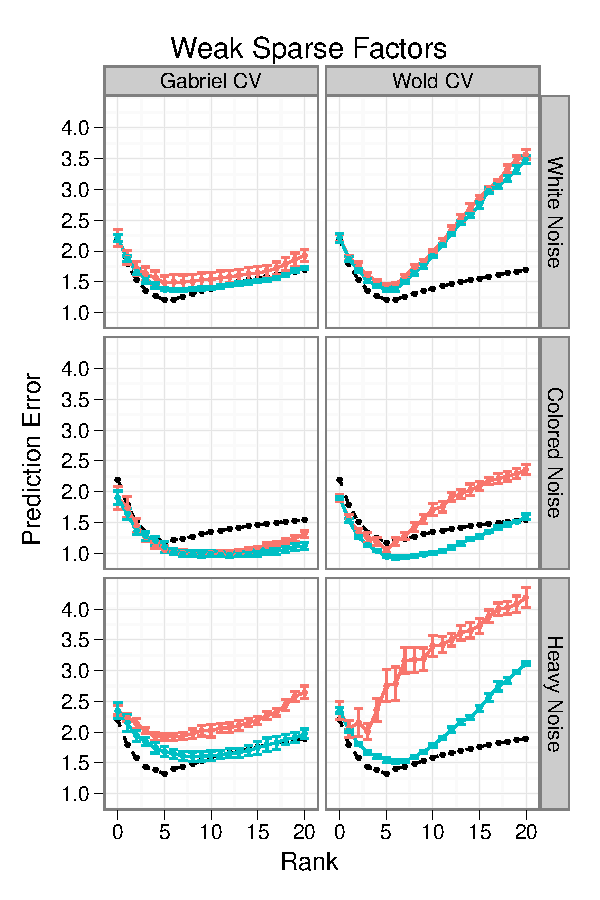
\includegraphics[scale=0.66]{cvsvd-weak-sparse}
        \end{center}
    \end{minipage}
    \caption{
        \captiontitle{Cross-validation with weak factors}
    }
\end{figure}

\begin{figure}[htb]
    \centering
    \begin{minipage}{0.49\textwidth}
        \begin{center}
            \includegraphics[scale=0.66]{cvsvd-strong-gauss}
        \end{center}
    \end{minipage}
    \begin{minipage}{0.49\textwidth}
        \begin{center}
            \includegraphics[scale=0.66]{cvsvd-strong-sparse}
        \end{center}
    \end{minipage}
    \caption{
        \captiontitle{Cross-validation with strong factors}
    }
\end{figure}


\clearpage

\begin{figure}[tbh]
    \centering
    \begin{minipage}{0.38\textwidth}
        \begin{center}
            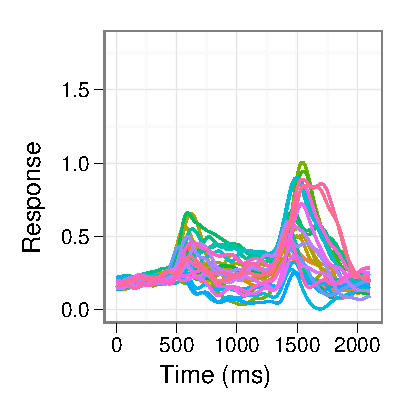
\includegraphics{neuron1}
        \end{center}
    \end{minipage}
    \begin{minipage}{0.61\textwidth}
        \begin{center}
            \includegraphics{neurons}
        \end{center}
    \end{minipage}
    \caption{
        \captiontitle{Motor Cortex Data}
        Response rates in 47 neurons for 27 movement tasks.  The subplots show
        the normalized response rates in a single neuron as functions of time.  
        Each color corresponds to a different movement task.  The plot on
        the left is a zoomed-in view of the data for the first neuron.
    }
\end{figure}
